\documentclass{article}
\usepackage[utf8]{inputenc}
\usepackage{amsthm}
\usepackage{amsmath}
\usepackage{amssymb}
\usepackage{tikz}
\usepackage{authblk}

\usetikzlibrary{calc,shapes.geometric}

\newtheorem*{definition}{Definition}
\newtheorem*{proposition}{Proposition}
\newtheorem*{lemma}{Lemma}

\newcommand{\R}{\mathbb{R}}
\newcommand{\pwrset}{\mathcal{P}}

\newcommand{\B}{\mathcal{B}}
\newcommand{\bcup}{\cup}
\newcommand{\bcap}{\Cap}
\newcommand{\bstar}{^\circledast}
\newcommand{\bcont}{\mathcal{C}^\R}
\newcommand{\bmeasure}{\leq_\mu^\R}

\newcommand{\lang}{\mathcal{L}}
\newcommand{\Vars}{\text{Vars}}
\newcommand{\Pol}{\text{Pol}}


\newcommand{\lcup}{\sqcup}
\newcommand{\lcap}{\sqcap}
\newcommand{\lstar}{^*}
\newcommand{\lpart}{\sqsubseteq}
\newcommand{\lcont}{C}
\newcommand{\lmeasure}{\preceq}

\newcommand{\eqdef}{\stackrel{\text{def}}{=}}

\title{Axiomatization of Some Contact Logics with a Qualitative Measure}
\author{Anguel Nikolov\\{\small supervised by Prof. Tinko Tinchev}}
\affil{Faculty of Mathematics and Informatics \\
  Sofia University ``St. Kliment Ohridski''}
\date{2021}

\begin{document}

\maketitle

\tableofcontents

\section{Introduction}

The aim of this work is to explore the axiomatization and decidability of the quantifier-free theories of a structure, which arises from a certain kind of geometric objects on the real line. Three relations between these objects are considered: parthood, contact and qualitative measure.

The objects are referred to as polytopes, though they are in fact unions of what may usually be understood by the term. A key property by which they are chosen is that they have a true interior.

The parthood relationship between these objects gives rise to a Boolean algebra and two further relations are considered --- those of contact and of qualitative measure.

\section{Language}
This section describes the language, whose semantics we will consider in a couple of contexts.

\begin{definition}[Language]
$\lang$ denotes the first-order language of only quantifier-free formulas, which contains the following non-logical symbols:
\begin{itemize}
  \item predicate symbols:
  \begin{itemize}
  \item binary infix $\lpart$: parthood
  \item binary infix $\lmeasure$: measure comparison
  \item binary prefix $\lcont$: contact
  \end{itemize}
  \item functional symbols:
  \begin{itemize}
  \item binary infix function $\lcup$: union
  \item binary infix function $\lcap$: intersection
  \item unary postfix function $\lstar$: complement
  \end{itemize}
  \item constant symbols:
  \begin{itemize}
  \item $0$: empty polytope
  \item $1$: universe
  \end{itemize}
\end{itemize}

The logical symbols $\land$, $\lor$, $\lnot$, $\Rightarrow$, $\top$, $\bot$ are used in the usual way and the set of individual variables is denoted $\Vars$.

\end{definition}

\section{Semantics}

Though the aim is to interpret the language on the real line, other models will also be needed. It is beneficial fix their common semantics, which are defined below in the expected way.

Let $\B$ be a Boolean algebra with carrier $B$ and $\mathcal{C}$ and $\mathcal{M}$ --- relations over $B$. Further, $S = \langle \B, \mathcal{C}, \mathcal{M} \rangle$.

\begin{definition}[Value of a Term in $S = \langle \B, \mathcal{C}, \mathcal{M} \rangle$]
  Let $v: \Vars \rightarrow B$. Then,  $v^S$ denotes the extension of $v$ to the terms of $\lang$ in the following structurally recursive way:
  \begin{itemize}
  \item $v^S(0)$ is the zero of $\B$
  \item $v^S(1)$ is the unit of $\B$
  \item $v^S(\tau_1 \lstar)$ is the complement of $v(\tau_1)$ in $\B$,
  \item $v^S(\tau_1 \lcup \tau_2)$ is the join of $v(\tau_1)$ and $v(\tau_2)$ in $\B$,
  \item $v^S(\tau_1 \lcap \tau_2)$ is the meet of $v(\tau_1)$ and $v(\tau_2)$ in $\B$,
  \end{itemize}
for any terms $\tau_1$ and $\tau_2$ of $\lang$.

\end{definition}

\begin{definition}[Validity of a Formula in $S = \langle \B, \mathcal{C}, \mathcal{M} \rangle$]
  Again, let $v: \Vars \rightarrow B$. Validity of a formula $\phi$ in $S$ with valuation $v$ is denoted $\langle S, v \rangle \models \phi$ and defined over elementary formulas like so:
  \begin{itemize}
  \item $\langle S, v \rangle \models \tau_1 \lpart \tau_2 \longleftrightarrow v^S(\tau_1)$ is less than or equal to $v^S(\tau_2)$ in $\B$,
  \item $\langle S, v \rangle \models \lcont(\tau_1, \tau_2) \longleftrightarrow \mathcal{C}(v^S(\tau_1), v^S(\tau_2))$,
  \item $\langle S, v \rangle \models \tau_1 \lmeasure \tau_2 \longleftrightarrow \mathcal{M}(v^S(\tau_1), v^S(\tau_2))$,
  \end{itemize}
  for any terms $\tau_1$ and $\tau_2$ of $\lang$. For complex formulas, the extension is done in the usual way:
  \begin{itemize}
  \item $\langle S, v \rangle \models \top$ and $\langle S, v \rangle \not \models \bot$,
  \item $\langle S, v \rangle \models \lnot \phi \longleftrightarrow \langle S, v \rangle \not\models \phi$,
  \item $\langle S, v \rangle \models \phi \land \psi \longleftrightarrow \langle S, v \rangle \models \phi$ and $\langle S, v \rangle \models \psi$,
  \item $\langle S, v \rangle \models \phi \lor \psi \longleftrightarrow$ at least one of  $\langle S, v \rangle \models \phi$ and $\langle S, v \rangle \models \psi$ holds,
  \end{itemize}
  where $\phi$ and $\psi$ are (quantifier-free) formulas of $\lang$.

  If $\langle S, v \rangle \models \phi$ for all $v: \Vars \rightarrow B$, then $S \models \phi$.
\end{definition}

\subsection{Polytopes on the Real Line}

A specific kind of objects will be considered --- finite unions of closed, potentially infinte, intervals on the real line. These are defined below, along with the operations and properties with which the language will be concerned.

\begin{definition}[Basis Polytope]
For any $m$, $n \in \mathbb{R}$, such that $m < n$, the intervals $[m, n]$, $(-\infty, m]$, $[m, \infty)$ and $(-\infty, \infty)$ are called \emph{basis polytopes}.
\end{definition}

Note that in the above definition and throughout the rest of the text, $-\infty$ and $\infty$ are used in the usual way --- as the least and the greatest elements of $\R \cup \{-\infty, \infty\}$.

\begin{definition}[Polytope]
For any finite set of basis polytopes $B$, $\bigcup B$ is called a \emph{polytope}. The set of all polytopes is denoted $\Pol(\R)$.
\end{definition}

Remark that for $B = \emptyset$, the empty set is also a polytope.

\begin{proposition}
Any non-empty polytope can be uniquely represented as the union of a finite set of non-intersecting basic polytopes.
\end{proposition}
\begin{proof}
  \textbf{TODO: write proof.}
\end{proof}

\begin{definition}(Standard Representation)
The set from the above proposition is the \emph{standard representation} of a polytope.
\end{definition}

\begin{definition}[Polytope Operations]
For any polytopes $p$ and $q$, we define the following operations as modifications of intersection and complement:
\begin{itemize}
  \item $p \bcap q \eqdef Cl(Int((p \cup q)))$;
  \item $p \bstar \eqdef Cl(\R \setminus p) $.
\end{itemize}
The union operation $p \bcup q$ will be considered in the same context, though no modification is needed.
\end{definition}

The modification of union ensures that there are no isoltated points and the modification of complement --- that results of the operations remain a union of \emph{closed} intervals.

\begin{proposition}
$\Pol(\R)$ forms a Boolean algebra with
\begin{itemize}
  \item $\bcap$ for meet,
  \item $\bcup$ for join,
  \item $\bstar$ for complement,
  \item $\emptyset$ for the zero and
  \item $\R$ for the unit.
\end{itemize}
This algebra will be denoted $\B^\R$.
\end{proposition}
\begin{proof}
  \textbf{TODO: write proof.}
\end{proof}

\begin{definition}[Line Contact]
Two polytopes $p$ and $q$ are \emph{in contact} if $p \cap q \neq \emptyset$. This is denoted $\bcont(p, q)$.
\end{definition}

\begin{definition}[Measure]
  The measure of a basic polytope of the kind $[m, n]$ is $n-m$. The measure of a basic polytope with an infinite bound is $\infty$.

  The \emph{measure} of a polytope $p$, denoted $\mu^\R(p)$ is $\infty$, if one of the polytopes of its standard representation has measure $\infty$, or their sum otherwise.

Further and most importantly, the \emph{qualitative measure relation induced by} $\mu^\R$ is defined
\begin{equation*}
  p \bmeasure q \longleftrightarrow \mu^\R(p) \leq \mu^\R(q),
\end{equation*}
  for any $p, q \in \Pol(\R)$.
\end{definition}

This definition is fully in line with the usual measure-theoretic one. Remark that the only polytope with measure $0$ is $\emptyset$. Further, every non-zero polytope has an arbitrary small non-zero sub-polytope.
Now, the model on the real line is defined as
\begin{definition}[Real Line Model]
  \begin{equation*}
    S^\R \eqdef \langle \B^\R, \bcont, \bmeasure \rangle
  \end{equation*}
\end{definition}

\subsection{Relational Models}
In order to find appropriate value functions for a well chosen kind of formulas, an abstraction model will be needed. It is quite generic, yet it turns out to be easily transformed into an equivalent real line model, given some constraints.

Let $W$ be a finite set and $\B^W$ --- the Boolean algebra of all subsets of $W$. Let $c$ be an arbitrary symmetric and reflexive relation over $W$ and $m: W \rightarrow \R^+ \cup \{\infty\}$.

Let $\mathcal{C}^c$ be the relation over $\pwrset(W)$ defined as
\begin{equation*}
  \mathcal{C}^c(a, b) \longleftrightarrow (\exists i \in a)(\exists j \in b)(\langle i, j \rangle \in c)
\end{equation*}
Let $\mu^m: \pwrset(W) \rightarrow \R_0^+ \cup \{\infty\}$ such that:
\begin{equation*}
  \mu^m(a) \eqdef
  \begin{cases}
    \infty           & \text{if $(\exists i \in a)(m(i) = \infty)$} \\
    \sum_{i \in a}m(i) & \text{otherwise}
  \end{cases}
\end{equation*}
And finally, let $\leq_m$ be the relation over $\pwrset(W)$:
\begin{equation*}
  a \leq_m b \longleftrightarrow \mu^m(a) \leq \mu^m(b),
\end{equation*}
all for $a$, $b \subseteq W$.
\begin{definition}[Relational Model]
$\langle \B^W, \mathcal{C}^c, \leq_m \rangle$ is called the \emph{relational model for $W$, $c$ and $m$}.
\end{definition}

\subsubsection{Converting to a Real Line Model}
Relational models are useful because they can be converted to real line models under certain conditions.
\begin{definition}[Contact Graph]
  Let $S = \langle \B^W, \mathcal{C}^c, \leq_m \rangle$ be a relational model. Let $E$ denote the set of pairs of different vertices in $c$, but unordered: $E \eqdef \{\, \{i, j\} \mid \langle i, j \rangle \in c$ \& $i \neq j \,\}$. Note that since $c$ is reflexive and symmetric, no information is lost when moving to $E$.
  The graph $\langle W, E \rangle$ is called the \emph{contact graph} of $S$ and denoted $Gr(S)$.
\end{definition}
\begin{definition}[Convertable Relational Model]
Let $S = \langle \B^W, \mathcal{C}^c, \leq_m \rangle$ be a relational model and suppose that the following constraints hold:
\begin{itemize}
\item $Gr(S)$ is connected and
\item there are exactly two elements of $W$ with infinite values for $m$, i.e. there exist $i \in W$ and $j \in W$, $i \neq j$, such that:
  \begin{equation*}
    m(i) = m(j) = \infty \text{ and } (\forall k \in W \setminus \{i, j\})(m(k) \neq \infty).
  \end{equation*}
\end{itemize}
Then, $S$ is called a \emph{convertable relational model}.
\end{definition}

\begin{definition}[Disjoint Valuation]
  Suppose $S = \langle \B^W, \mathcal{C}^c, \leq_m \rangle$ is a convertable relational model and $v: \Vars \rightarrow \pwrset(W)$, such that
\begin{equation*}
(\forall x \in \Vars)(\forall y \in \Vars)(v(x) \neq v(y) \rightarrow v(x) \cap v(y) = \emptyset).
\end{equation*}
Then, $v$ is called a \emph{disjoint valuation}.
\end{definition}

\begin{lemma}[Untying]
  Let $S = \langle \B^W, \mathcal{C}^c, \leq_m \rangle$ be a convertable relational model and $v$ --- a disjoint valuation. Suppose $Gr(S)$ is not a tree.
  Then, there is a procedure to effectively compute a convertable relational model $S'$ and a disjoint valuation $v'$ for $S'$ in polynomial time, so that:
  \begin{itemize}
  \item $Gr(S')$ has one vertex more and the same number of edges and
  \item for any formula $\phi$ in $\lang$, $\langle S, v \rangle \models \phi \longleftrightarrow \langle S', v' \rangle \models \phi$.
  \end{itemize}
\end{lemma}
\begin{proof}
  Given that $Gr(S)$ is not a tree, yet is connected, it must contain at least one cylce. A cycle can be effectively found in polynomial time using a depth-first search. Let $\pi$ be such a cycle.

  Let $i$ and $j$ be any two consecutive vertices in $\pi$, such that $m(i) \neq \infty$. This requirement is always achievable, since there are at least three vertices in a cycle and exactly two vertices with infinte values for $m$ in a convertable relational model. Therefore, there will be at least one vertex with a finite value for $m$ in any cycle.

  The intuition behind the method for removing the edge between $i$ and $j$ is that the portion which is in contact only with $j$ of the atomic object $i$ is being separated out into a separate atomic object, having half the measure.

\begin{figure}[h]
    \centering
    \begin{minipage}{0.45\textwidth}
      \centering
      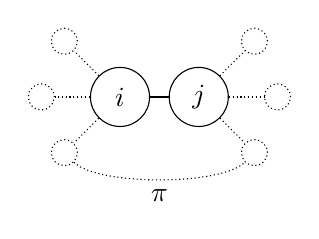
\begin{tikzpicture}[main/.style = {draw, circle, minimum size=.75cm},
          small/.style = {draw, densely dotted, circle, minimum size=.25cm},
          dedge/.style = {densely dotted}]
        \node[main] (i) {$i$};
        \node[main] (j) [right of=i] {$j$};
        \node[small] (i1) [below left of=i] {};
        \node[small] (i2) [above left of=i] {};
        \node[small] (i3) [left of=i] {};
        \node[small] (j1) [below right of=j] {};
        \node[small] (j2) [above right of=j] {};
        \node[small] (j3) [right of=j] {};
        \draw (i) -- (j);
        \foreach \n in {i1, i2, i3}
                 {
                   \draw[dedge] (i) -- (\n);
                 }
        \foreach \n in {j1, j2, j3}
                 {
                   \draw[dedge] (j) -- (\n);
                 }
        \draw[dedge] (i1) to [out=315, in=225, looseness=.5] node[midway, below] {$\pi$} (j1);
      \end{tikzpicture}
    \end{minipage}$\rightsquigarrow$
    \begin{minipage}{0.45\textwidth}
      \centering
      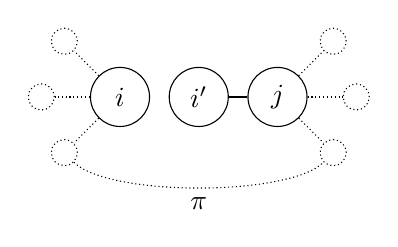
\begin{tikzpicture}[main/.style = {draw, circle, minimum size=.75cm},
          small/.style = {draw, densely dotted, circle, minimum size=.25cm},
          dedge/.style = {densely dotted}]
        \node[main] (i) {$i$};
        \node[main] (i') [right of=i] {$i'$};
        \node[main] (j) [right of=i'] {$j$};
        \node[small] (i1) [below left of=i] {};
        \node[small] (i2) [above left of=i] {};
        \node[small] (i3) [left of=i] {};
        \node[small] (j1) [below right of=j] {};
        \node[small] (j2) [above right of=j] {};
        \node[small] (j3) [right of=j] {};
        \draw (i') -- (j);
        \foreach \n in {i1, i2, i3}
                 {
                   \draw[dedge] (i) -- (\n);
                 }
        \foreach \n in {j1, j2, j3}
                 {
                   \draw[dedge] (j) -- (\n);
                 }
%        \draw[dedge] (i1)  (j1);
        \draw[dedge] (i1) to [out=315, in=225, looseness=.5] node[midway, below] {$\pi$} (j1);
      \end{tikzpicture}
    \end{minipage}
\end{figure}

  Let $i' \not \in W$ and let:
\begin{align*}
W' &\eqdef W \cup \{i'\} \\
c' &\eqdef (c \setminus \{\langle i, j \rangle, \langle j, i \rangle\}) \cup \{\langle i', j \rangle, \langle j, i' \rangle, \langle i', i' \rangle\} \\
m'(k) &\eqdef \begin{cases}
m(k)           & \text{if $k \not \in \{i, i'\}$} \\
m(i) / 2       & \text{otherwise}
\end{cases}\text{, for any } k \in W'. \\
S' &\eqdef \langle \B^{W'}, \mathcal{C}^{c'}, \leq_{m'} \rangle \\
v'(x) &\eqdef \begin{cases}
  v(x) \cup \{i'\} & \text{if } i \in v(x) \\
  v(x)             & \text{otherwise}
\end{cases}\text{, for any } x \in \Vars.
\end{align*}

Note that the construction of $S'$ and $v'$ happens in polynomial time --- it consists of copying $S$ and $v$, except for a small number of changes not dependent on the size of $S$.

\textbf{TODO: $v'$ is not a finite object. It is stupid to say it can be effectively constructed. Figure out how to cleanly avoid this.}

It is directly clear that $S'$ is a relational model. Compared to $S$, there is one more vertex in $Gr(S')$ and the same number of edges ($\{i, j\}$ is removed, $\{i', j\}$ is added).

Any path between two vertices in $Gr(S)$ corresponds to a path in $Gr(S')$, by potentially substituting the edge $\{i, j\}$ for the detour path along $\pi$. Therefore, all vertices in $W$ are connected in $Gr(S')$. $i'$ is connected to $i$ and from there to the rest of $W$ as well, so $Gr(S')$ is connected.

$m'$ has the same values as $m$ over all elements of $W'$, except $i$ and $i'$, where it's values are finite. Therefore, the same two elements of $W'$ that have infinite values for $m$, also have infinte values for $m'$ and no others.

Thus, $S'$ is a convertable relational model.

To demonstrate by contraposition that $v'$ is a disjoint valuation, let $x \in \Vars$, $y \in \Vars$ and assume that $v'(x) \cap v'(y) \neq \emptyset$. Let $k \in v'(x) \cap v'(y)$, for some $k \in W'$. If $k = i'$, $i' \in v'(x)$, so $i \in v(x)$ by the definition of $v'$. Analagously, $i \in v(y)$ and $v(x) \cap v(y) \neq \emptyset$. On the other hand, if $k \neq i'$, again by the definition of $v'$, $k \in v(x) \cap v(y)$. In both cases, since $v$ is a disjoint valuation and $v(x) \cap v(y) \neq \emptyset$, $v(x) = v(y)$. From here, $v'(x) = v'(y)$ and $v'$ is a disjoint valuation.

Now follows a proof by induction on terms in $\lang$, that
\begin{equation*}
  v'^{S'}(\tau) =
  \begin{cases}
    v^S(\tau)             & \text{if } i \in v^S(\tau) \\
    v^S(\tau) \cup \{i'\} & \text{otherwise}
  \end{cases}
  \text{, for any term } \tau \text{ of } \lang.
\end{equation*}
\begin{itemize}
  \item For the two constants $0$ and $1$,
    \begin{equation*}
      v'^{S'}(0) = \emptyset = v^S(0) \text{ and } i \not \in v^S(0)
    \end{equation*}
    \begin{equation*}
      v'^{S'}(1) = W' = W \cup \{i'\} = v^S(1) \cup \{i'\} \text{ and } i \in v^S(1)
    \end{equation*}
  \item For terms consisting of individual variables, the statement holds by the definition of $v'$.
  \item Suppose, as induction hypothesis, that the statement holds for $\tau_1$ and $\tau_2$.
    \begin{itemize}
    \item To show that the statement holds for $\tau_1 \lcup \tau_2$, suppose first that $i \in v^S(\tau_1 \lcup \tau_2)$. Then, $i \in v^S(\tau_1) \cup v^S(\tau_2)$ and $i \in v^S(\tau_1)$ or $i \in v^S(\tau_2)$. Without loss of generality, assume $i \in v^S(\tau_1)$. By induction hypothesis, $v'^{S'}(\tau_1) = v^S(\tau_1) \cup \{i'\}$ and $v'^{S'}(\tau_2) \subseteq v^S(\tau_2) \cup \{i'\}$. Thus, $v'^{S'}(\tau_1 \lcup \tau_2) \eqdef v'^{S'}(\tau_1) \cup v'^{S'}(\tau_2) = v^S(\tau_1) \cup v^S(\tau_2) \cup \{i'\} \eqdef v^S(\tau_1 \lcup \tau_2) \cup \{i'\}$.

      Alternatively, suppose $i \not \in v^S(\tau_1 \lcup \tau_2)$. Then, $v'^{S'}(\tau_1 \lcup \tau_2) \eqdef v'^{S'}(\tau_1) \cup v'^{S'}(\tau_2) = v^S(\tau_1) \cup v^S(\tau_2) \eqdef v^S(\tau_1 \lcup \tau_2)$ directly, using the induction hypothesis.

    \item To show that the statement holds for $\tau_1 \lcap \tau_2$, suppose $i \in v^S(\tau_1 \lcap \tau_2)$. Then, $i \in v^S(\tau_1) \cap v^S(\tau_2)$, so $i \in v^S(\tau_1)$ and $i \in v^S(\tau_2)$. By induction hypothesis, $v'^{S'}(\tau_1) = v^S(\tau_1) \cup \{i'\}$ and $v'^{S'}(\tau_2) = v^S(\tau_2) \cup \{i'\}$. Thus, $v'^{S'}(\tau_1 \lcap \tau_2) \eqdef v'^{S'}(\tau_1) \cap v'^{S'}(\tau_2) = (v^S(\tau_1) \cup \{i'\}) \cap (v^S(\tau_2) \cup \{i'\}) = (v^S(\tau_1) \cap v^S(\tau_2)) \cup \{i'\} \eqdef v^S(\tau_1 \lcup \tau_2) \cup \{i'\}$.

      Alternatively, if $i \not \in v^S(\tau_1 \lcap \tau_2)$. $i \not \in v^S(\tau_1) \cap v^S(\tau_2)$. Using the induction hypothesis, $v'^{S'}(\tau_1 \lcap \tau_2) \eqdef v'^{S'}(\tau_1) \cap v'^{S'}(\tau_2) = v^S(\tau_1) \cap v^S(\tau_2) \eqdef v^S(\tau_1 \lcap \tau_2)$.

    \item To show the statement holds for $\tau_1\lstar$, consider that $v'^{S'}(\tau_1\lstar) \eqdef W' \setminus v'^{S'}(\tau_1) \eqdef (W \cup \{i'\}) \setminus v'^{S'}(\tau_1)$.

      Suppose $i \in v^S(\tau_1\lstar)$. By induction hypothesis, $(W \cup \{i'\}) \setminus v'^{S'}(\tau_1) = (W \cup \{i'\}) \setminus (v^S(\tau_1) \cup \{i'\}) = W \setminus v^S(\tau_1) \eqdef v^S(\tau_1\lstar)$.

      Alternatively, if $i \not \in v^S(\tau_1\lstar)$, $(W \cup \{i'\}) \setminus v'^{S'}(\tau_1) = (W \cup \{i'\}) \setminus v^S(\tau_1) = (W \setminus v^S(\tau_1)) \cup \{i'\} \eqdef v^S(\tau_1\lstar) \cup \{i'\}$.
    \end{itemize}
\end{itemize}
Now to demonstrate that for any formula $\phi$ in $\lang$, $\langle S, v \rangle \models \phi \longleftrightarrow \langle S', v' \rangle \models \phi$ by induction on the construction of $\phi$, let $\tau_1$ and $\tau_2$ be terms of $\lang$.
\begin{itemize}
  \item For $\bot$ and $\top$, the statement is trivial.
  \item For parthood atomic formulas:
    \begin{itemize}
    \item If $i \in v^S(\tau_2)$,
      \begin{align*}
        \langle S, v \rangle \models \tau_1 \lpart \tau_2 &\longleftrightarrow \\
        v^S(\tau_1) \subseteq v^s(\tau_2) &\longleftrightarrow \\
        v^S(\tau_1) \cup \{i'\} \subseteq v^S(\tau_2) \cup \{i'\} &\longleftrightarrow \\
        v'^{S'}(\tau_1) \subseteq v'^{S'}(\tau_2) &\longleftrightarrow \\
        \langle S', v' \rangle \models \tau_1 \lpart \tau_2
      \end{align*}
    \item conversly, if $i \not \in v^S(\tau_2)$,
      \begin{align*}
        \langle S, v \rangle \models \tau_1 \lpart \tau_2 &\longleftrightarrow \\
        v^S(\tau_1) \subseteq v^s(\tau_2) &\longleftrightarrow \\
        v'^{S'}(\tau_1) \subseteq v'^{S'}(\tau_2) &\longleftrightarrow \\
        \langle S', v' \rangle \models \tau_1 \lpart \tau_2
      \end{align*}

    \end{itemize}
  \item To prove the statement for contact atomic formulas in one direction, assume that $\langle S, v \rangle \models \lcont(\tau_1, \tau_2)$. From here, $(\exists k \in v^S(\tau_1))(\exists l \in v^S(\tau_2))(\langle k, l \rangle \in c)$.
    Let $k_0$ and $l_0$ be witnesses for the variables $k$ and $l$.
    \begin{itemize}
    \item Suppose $\{k_0, l_0\} = \{i, j\}$. Without loss of generality, $k_0 = i$ and $l_0 = j$. Then, since $i \in v^S(\tau_1)$, $i' \in v'^{S'}(\tau_1)$ must hold. Further, $j \in v'^{S'}(\tau_2)$ and $\langle i', j \rangle \in c'$, so $\langle S', v' \rangle \models \lcont(\tau_1, \tau_2)$.
    \item Alternatively, if $\{k_0, l_0\} \neq \{i, j\}$, then $\langle k_0, l_0 \rangle \in c'$ (because $\langle k_0, l_0 \rangle \in c$), $k_0 \in v'^{S'}(\tau_1)$ and $l_0 \in v'^{S'}(\tau_2)$, so $\langle S', v' \rangle \models \lcont(\tau_1, \tau_2)$.
    \end{itemize}
    In the opposite direction, assume $\langle S', v' \rangle \models \lcont(\tau_1, \tau_2)$. Then, $(\exists k \in v'^{S'}(\tau_1))(\exists l \in v'^{S'}(\tau_2))(\langle k, l \rangle \in c')$. Again, let $k_0$ and $l_0$ be witnesses.
    \begin{itemize}
    \item Suppose $\{k_0, l_0\} = \{i', j\}$. Just as before, without loss of generality, $k_0 = i'$ and $l_0 = j$. Then, since $i' \in v'^{S'}(\tau_1)$, $i \in v^S(\tau_1)$ must hold. Further, $j \in v^S(\tau_2)$ and $\langle i, j \rangle \in c$, so $\langle S, v \rangle \models \lcont(\tau_1, \tau_2)$.
    \item
      Alternatively, suppose $\{k_0, l_0\} \neq \{i', j\}$. Now, $k_0 = i'$ and $l_0 = i'$ are both impossible, since $j$ is the only vertex in $W'$, connected to $i'$ by $c'$ and by assumption, $\{k_0, l_0\} \neq \{i', j\}$.

      Therefore, $k_0 \in W$, $l_0 \in W$, $k_0 \in v^S(\tau_1)$, $l_0 \in v^S(\tau_2)$ and $\langle k_0, l_0 \rangle \in c$, so $\langle S, v \rangle \models \lcont(\tau_1, \tau_2)$.
    \end{itemize}
\end{itemize}
\end{proof}

\begin{lemma}[Relational Model Conversion]
  Let $S = \langle \B^W, \mathcal{C}^c, \leq_m \rangle$ be a convertable relational model and $v$ --- a disjoint valuation. If $\phi$ is a formula from $\lang$ and $\langle S, v \rangle \models \phi$, then there exists $v^\R: \Vars \rightarrow \Pol(\R)$, such that $\langle S^\R, v^\R \rangle \models \phi$.
\end{lemma}
\begin{proof}
  \textbf{TODO: write proof.}
\end{proof}
\section{Axiomatization}
\subsection{Corectness}
\subsection{Completeness}
\subsection{Finite Axiomatization}
\end{document}
